\section{Related work}

Procedural terrain generation spans a spectrum from purely noise-driven algorithms to physics-based simulations and, more recently, data-driven methods. In the context of coral reef islands, where both long-term geological subsidence and biogenic reef accretion interplay, existing approaches fall short in one of two ways: either they lack ecological or geological grounding, or they offer insufficient authoring control.

\paragraph{Procedural and simulation-based methods}
Noise-based techniques such as Perlin noise (\cite{Perlin1985}), Simplex noise (\cite{Perlin2001}), and the Diamond-Square algorithm (\cite{Fournier1982}) (often extended via fBm or multifractal noise (\cite{Musgrave1989,Ebert2003})) remain popular for their simplicity and speed. Island shapes are generated by modulating noise with radial falloff masks (\cite{Olsen2004}), but these methods cannot reproduce reef rings, lagoons, or atoll structures in a geologically coherent manner. They treat terrain purely as a signal-processing problem, separated from processes like volcanic subsidence or coral growth (\cite{Smelik2009,Galin2019}).

Simulation-based approaches introduce surface deformations by modeling erosion (\cite{Benes2006,Neidhold2005,Mei2007}), tectonic uplift (\cite{Cordonnier2016,Cordonnier2017a,Schott2023}), or vegetation-terrain feedback (\cite{Ecormier-Nocca2021,Cordonnier2017b}). Hydraulic and thermal erosion capture fluvial networks and slope-driven mass wasting, but they omit underwater sedimentation and biogenic carbonate accretion. Tectonic and isostatic models excel at orogeny but ignore coral reef dynamics, while vegetation-based methods do not generalize to marine ecosystems. Consequently, none of these simulations jointly capture the slow subsidence of volcanic islands and the compensatory growth of surrounding reefs on the timescales required for atoll formation.

\paragraph{Sketch-based terrain modeling}
Sketch-driven interfaces bridge user intent and procedural detail. Curve-based systems let users draw ridges, valleys, or coastlines that guide surface deformation and noise propagation (\cite{Gain2009,Hnaidi2010}). Constraint-based methods extend this by enforcing absolute elevation or slope values at control curves or points, solved via diffusion or fractal interpolation (\cite{Gasch2020,Talgorn2018}), and even gradient-domain editing for slope control (\cite{Guerin2022}). Semantic approaches encode high-level "terrain atoms" from a dictionary of primitives (\cite{Genevaux2015}) or interpret geological schematics into 3D models (\cite{Natali2012}). While these techniques grant artists fine-grained control, they typically lack ecological constraints and have not been tailored to marine biogeomorphology.

\paragraph{Learning-based terrain synthesis}
Deep generative models offer a way to learn complex patterns without explicit procedural rules. Unconditional GANs have been applied to digital elevation maps of mountains (\cite{WulffJensen2018}) and joint height-texture synthesis (\cite{Spick2019}), but their reliance on latent noise prevents precise layout control. Two-stage pipelines use an initial GAN for heightmaps and a conditional GAN for textures (\cite{Beckham2017}) or reverse the order (imagery-to-DEM) (\cite{Panagiotou2020}), yet still lack the ability to guide authoring.

Conditional GANs (cGANs) extend image-to-image translation methods such as pix2pix (\cite{Isola2017}) to terrain, enabling sketch- or label-map-conditioned generation. Prior work includes sketch-to-DEM translation for generic landforms (\cite{Guerin2017}) and sparse "altitude dot" conditioning (\cite{Voulgaris2021}), as well as cGANs that invert satellite imagery into elevation (\cite{Sisodia2022}). However, these models require extensive paired real-world datasets which are scarce for coral reef islands.

% \paragraph{Summary}
% In summary, noise-based and simulation-driven methods either lack biogeological realism or authoring control, while sketch-based systems neglect marine ecological constraints. Unconditional and two-stage GANs fail to offer semantic layout guidance, and existing cGAN-based terrain approaches are data-hungry or domain-agnostic. We address these gaps by combining sketch-based region maps with a pix2pix cGAN trained on procedurally generated coral island datasets, thereby enforcing geological coherence (subsidence and reef growth) while preserving user-driven design.

% \section{Related works}
% \subsection{Traditional terrain generation methods}
% \label{sec:coral-island_sota-traditional}

% Procedural generation of terrain has been a well-researched area in computer graphics and simulations, where the goal is to create large, realistic landscapes with minimal manual input. Various methods have been developed over the years to generate terrains automatically, from noise-based approaches to physically-based erosion simulations, sketch-driven methods, and more recently, deep learning techniques.

% However, each of these techniques has its strengths and limitations, particularly when it comes to modeling coral reef islands. Coral reef islands present unique challenges due to the combination of long-term geological processes (such as subsidence and coral reef growth) and environmental interactions (like erosion caused by wind and waves). In this section, we review the key techniques that have been applied to terrain generation, highlight their limitations for coral reef island formation, and position our work as an approach that addresses these challenges.


% \subsubsection{Noise-based terrain generation}

% \begin{figure}[ht]
%     \centering
%     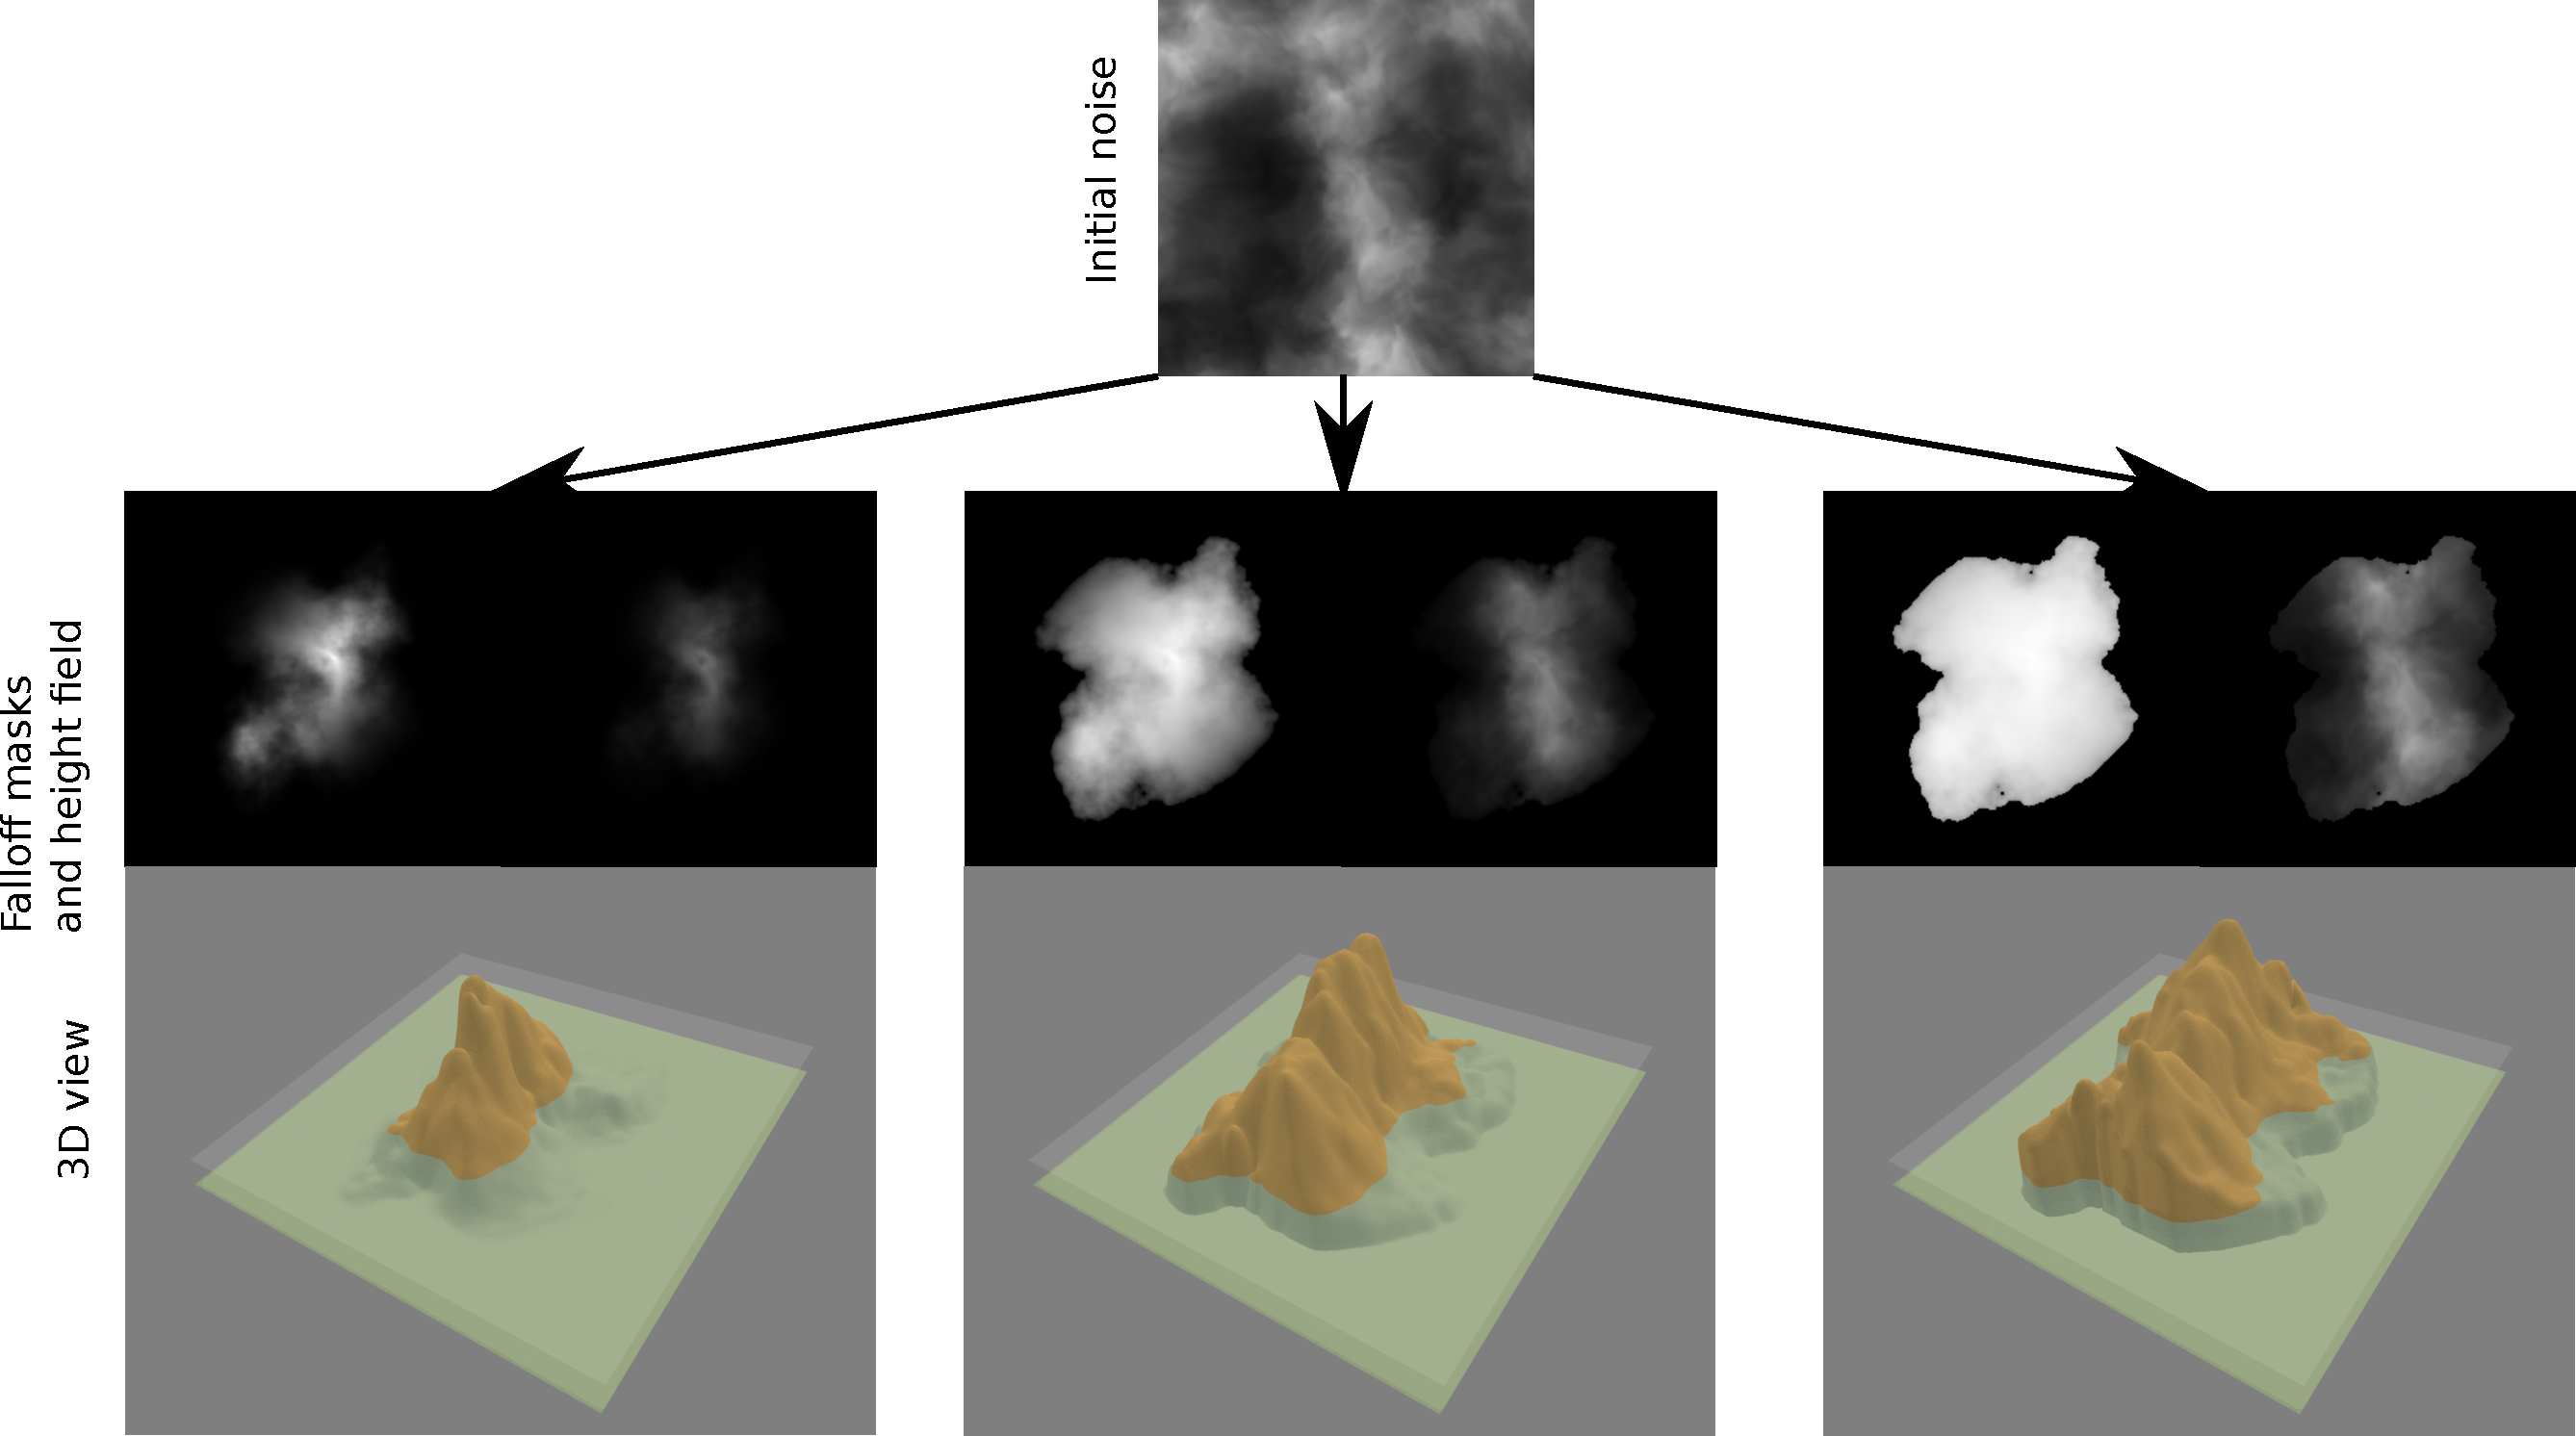
\includegraphics[width = \linewidth]{noise_examples3.pdf}
%     \caption{Three different results of an island generated from noise functions. In each case, the initial height field is the same, computed through flow noise. The falloff masks are also generated with a combination of fBm noise mitigated by the euclidean distance from the image center, warp noise and gamma correction. The only parameter modified for each example is the gamma correction. The results are very different, and hardly controllable. It is also difficult to represent lagoons and reefs using this method.}
%     \label{fig:coral-island_noise-example}
% \end{figure}

% Noise-based procedural generation remains one of the most widely used techniques for creating natural-looking terrains. Perlin noise (\cite{Perlin1985}), Simplex noise (\cite{Perlin2001}), and the Diamond-square algorithm (\cite{Fournier1982}) are foundational algorithms that generate pseudo-random yet continuous variations across a grid, producing terrain features that resemble organic landscapes. These techniques have been widely adopted in computer graphics and game development due to their efficiency and visual appeal.

% Beyond basic noise functions, more advanced techniques such as fractal Brownian motion (fBm) and multifractal noise have been introduced to add finer-scale variation and detail (\cite{Musgrave1989,Ebert2003}). FBm combines multiple layers, or "octaves," of noise at different frequencies and amplitudes, producing terrains that exhibit more realistic and varied features. The combination of noise with domain warping and signal processing techniques has been explored in depth in procedural modeling literature (\cite{Reinhard2010}), enabling further control over visual complexity and terrain realism.

% Noise functions are often paired with falloff maps to produce island-like terrains, where elevation gradually decreases toward the edges of the domain, mimicking coastlines and basic island shapes (see \cref{fig:coral-island_noise-example}). Various methods for enhancing island generation using noise and falloff blending have been proposed for applications in games and virtual worlds (\cite{Olsen2004}). While these techniques excel at producing large, visually diverse landscapes quickly, they suffer from several key limitations when applied to the modeling of coral reef islands.

% Critically, noise-based terrains lack grounding in geological or biological reality. They generate spatial patterns through mathematical noise, not through simulations of real-world processes such as volcanic subsidence or coral accretion. The signal processing parameters typically involved (frequency, lacunarity, gain, amplitude, ...) are tuned for visual effect rather than scientific plausibility. As highlighted in procedural modeling surveys (\cite{Smelik2009,Galin2019}), this disconnect results in a lack of semantic control and poor correlation with actual environmental dynamics, making it difficult to represent phenomena like reef rings, lagoons, or atoll structures in a biologically or geologically coherent way.

% Moreover, the biological aspects of coral growth are inherently tied to environmental conditions. Coral reefs form and persist only within specific ranges of water depth, sunlight, salinity, and water quality. Their growth patterns are further influenced by ecological health, nutrient availability, and symbiotic relationships. These dependencies are extremely difficult to capture in procedural noise systems, which are not designed to model such complex and coupled dynamics.

% Our approach goes beyond the randomness of noise-based generation by incorporating real-world geological and biological processes into the terrain formation pipeline. Specifically, we model the gradual subsidence of volcanic islands and the upward growth of coral reefs, both of which are central to the long-term evolution of coral reef islands. By embedding these natural processes directly into the generation algorithm, we produce terrains that are not only more realistic but also more controllable. This integration of scientific modeling with procedural flexibility allows us to overcome the inherent limitations of traditional noise-based techniques and more accurately represent the complex formation of coral reef island systems.

% \subsubsection{Simulation-based modeling}

% Simulation-based terrain modeling methods aim to increase realism by replicating natural processes such as erosion, sediment transport, tectonic uplift, and vegetation growth. Unlike noise-based techniques, which rely on random functions, simulation-based approaches model causality and temporal dynamics to describe how a terrain evolves over time under physical or biological forces. These methods are often used to enhance base terrains, adding geologically plausible detail and structure (\cite{Benes2006, Smelik2009}).

% \subsubsubsection{Hydraulic and thermal erosion}

% Hydraulic erosion models simulate the impact of flowing water on the landscape by modeling erosion, sediment pickup, transport, and deposition. Early implementations by (\cite{Musgrave1989}) laid the groundwork for erosion in procedural generation, while more recent works have accelerated these simulations using GPU architectures (\cite{Mei2007}) and particle-based methods (\cite{Neidhold2005}). These simulations often follow Eulerian fluid models or Lagrangian particle systems to capture terrain displacement.

% Thermal erosion, by contrast, simulates mass movement due to gravity, redistributing material from steeper slopes to gentler gradients, akin to landslides or soil creep (\cite{Benes2006}). These erosion models generate realistic fluvial networks and landforms, but they are parameter-sensitive and computationally expensive.

% Moreover, such models are generally designed for terrestrial landscapes and lack mechanisms for simulating underwater sedimentation, reef growth, or biogenic processes crucial to coral island formation. These models typically simulate time scales relevant to geomorphological processes (hundreds to thousands of years), which are mismatched with both the faster dynamics of biological processes like coral health and the slower geological evolution of reef islands.

% We will propose our new particle-based erosion simulation method, adapted for underwater and terrestrial landscapes, in \cref{chap:erosion}.

% \subsubsubsection{Tectonic uplift and geologic simulation}

% Geological simulation approaches such as those proposed by (\cite{Cordonnier2016, Cordonnier2017a}) and extended by (\cite{Schott2023}) model terrain evolution through crustal deformation and tectonic uplift. These methods simulate isostatic adjustments, plate tectonics, or local uplift phenomena, often over geological timescales.

% Although well-suited for mountain-building processes or fault line modeling, these methods are not designed to account for biogenic terrain formation, such as coral reef accretion, which is critical for simulating coral reef islands. As a result, despite being physically grounded models, they do not capture the coupled geological and biological dynamics necessary for representing the long-term evolution of reef islands.

% \subsubsubsection{Vegetation and ecosystem dynamics}

% Some simulation-based terrain models integrate ecological dynamics to reflect the feedback between terrain and living systems. For instance, ()\cite{Ecormier-Nocca2021}) and (\cite{Cordonnier2017b}) simulate interactions between vegetation and terrain erosion, modeling plant colonization, growth, and their influence on soil stability and moisture retention.

% These ecosystem simulations allow more complex landscape evolution by considering biotic agents; however, they are designed primarily for terrestrial plants and temperate ecosystems. Coral colonies, in contrast, are marine organisms with strict environmental requirements such as limited depth, adequate sunlight, warm water temperatures, and clear water for photosynthesis via symbiotic algae. Accurately simulating these dependencies would require significant computation resources.

% Furthermore, coral growth is not a passive process like sediment accumulation or root expansion, but an active accretion system that builds calcium carbonate structures over thousands of years. These unique growth mechanisms, constrained by marine ecology, fall outside the scope of existing vegetation or soil-plant-water feedback models.

% \midConclusion

% While simulation-based models represent a significant advancement over purely procedural approaches, they fall short in capturing the coupled geological and biological dynamics that shape coral reef islands. They are either computationally intensive, domain-specific, or biologically inapplicable, highlighting the need for a new class of terrain generation tools that embed long-term marine biogeomorphological processes into the procedural pipeline.




% \subsection{Sketch-based terrain modeling}
% \label{sec:coral-island_sota-sketches}

% The term sketching encompasses several meanings: it can refer to performing gestures with the hand or body, creating a rough drawing, or outlining an idea in a simplified form. Accordingly, sketch-based modeling in 3D computer graphics can be understood through three complementary perspectives, each centered around a distinct core concept.

% First, sketching may focus on interaction, where gestures captured through hand or body motion are used to manipulate virtual objects, often in immersive environments like virtual or augmented reality, drawing on established techniques such as sculpting and distortion (\cite{Olsen2009, Cook2009}). Second, it can involve construction, where simple geometric primitives (curves, parametric shapes, implicit surfaces, ...) are combined under constraints to build more complex models. Finally, sketching may center on interpretation, where the user draws strokes on a 2D canvas and the system analyzes their meaning to generate a plausible 3D model.

% While sketch-based modeling encompasses a wide range of techniques, including gesture-driven interaction in immersive environments, this work focuses primarily on the construction and interpretation aspects. In particular, construction serves as the foundation for procedural generation techniques using geometric primitives and constraints (addressed in this section), while interpretation becomes relevant when exploring data-driven approaches using deep learning to infer terrain structure from sketches (discussed in the following section). Interaction-based techniques, though significant in other contexts, fall outside the scope of this work. 

% To distinguish clearly between the different aspects addressed in this chapter, we will refer to the constructive approach as sketch-based, and to the interpretive, learning-driven approach as learning-based. It is important to note, however, that the boundaries between these categories are inherently blurry and often overlap in practice.

% In procedural terrain generation, sketch-based construction approaches enable users to shape landscapes by manipulating high-level geometric primitives through intuitive sketching interfaces. These methods allow the definition of key terrain features, such as mountains, valleys, and coastlines, by drawing their outlines on a two-dimensional canvas, which are then procedurally transformed into 2.5D or 3D terrain representations. This approach offers a high degree of artistic control, making it particularly effective for creative applications like video games and simulations, where modeling is primarily user-driven.

% \subsubsection{Curve-based modeling}

% Sketch-based terrain generation often begins with user-defined curves that act as high-level constraints to guide the shape of the terrain. These curves may represent silhouettes, ridgelines, valleys, or feature outlines. Once defined, they are interpreted by the system and translated into elevation changes through various computational techniques. This approach allows for intuitive control over large-scale landforms while maintaining a procedural foundation for terrain synthesis.

% \AltTextImage{
%     One of the earliest and most influential works in this domain is the system introduced by (\cite{Gain2009}), which enables users to sketch silhouettes, ridges, and spine curves to define complex terrain structures (\cref{fig:coral-island_Gain-2009}). The method employs multiresolution surface deformation and propagates wavelet-based noise from the sketched features to their surroundings, allowing users to generate detailed, natural-looking terrains from minimal input. This approach demonstrated the effectiveness of combining intuitive sketch input with procedural detail synthesis.
%     We draw direct inspiration from this work's dual-view sketching strategy, combining top-view and profile sketches, which closely aligns with our concentric curve and height-profile input approach.

%     Expanding on this idea, (\cite{Hnaidi2010}) proposed a technique based on diffusion equations. In their method, curves are annotated with geometric constraints such as elevation or slope, and a diffusion process is used to interpolate these constraints across the terrain surface. This results in smooth, continuous elevation fields that conform to user-defined features such as rivers, ridgelines, or cliffs. The use of parameterized curves as terrain anchors allows for precise control over landform shaping, while maintaining a high degree of automation.
% }{sketchingGain2009-vertical.png}{caption}{fig:coral-island_Gain-2009}

% \AltTextImage{
%     In a different interaction paradigm, (\cite{Tasse2014}) introduced a first-person sketching interface, where users draw terrain silhouettes from a particular camera viewpoint (\cref{fig:coral-island_Tasse-2014}). These silhouettes are then projected into 3D, and a deformation algorithm adjusts the terrain so that the drawn features are visible exactly as intended from the user's perspective. This method supports complex silhouettes with occlusions, T-junctions, and cusps, and represents a more immersive and perceptually grounded approach to sketch-based terrain editing.
% }{sketchingTasse2014-vertical.png}{caption}{fig:coral-island_Tasse-2014}

% These methods demonstrate the expressive power of curves as terrain-defining elements. By enabling users to sketch intuitive shapes and constraints, they bridge the gap between artistic intent and procedural complexity. Curve-driven approaches remain foundational in terrain modeling, particularly when user control over large-scale structure is essential. While we do not use the diffusion model, the idea of sketch-defined elevation constraints along curves informs our use of user-defined shape boundaries.


% \subsubsection{Constraint-based modeling}

% While curve-driven techniques provide intuitive shape design, constraint-based and gradient-based approaches focus on exerting precise control over terrain features through formal specifications such as elevation values, slopes, or gradient fields. These methods prioritize structural accuracy and procedural consistency, making them particularly suited to applications that demand terrain realism, integration with geographic data, or fine-grained editing capabilities.

% \AltTextImage{
%     A representative example of constraint-based modeling is presented by (\cite{Gasch2020}), who propose a method for procedural terrain generation that respects user-defined elevation constraints (\cref{fig:coral-island_Gasch-2020}). Their system allows users to fix values at specific control points (e.g., paths, landmarks) and then employs a system of equations to propagate these constraints throughout the terrain. Crucially, the method integrates these constraints with a noise-based procedural function to preserve natural randomness while conforming to user intent. This approach is especially valuable when generating terrains that must align with real-world data or gameplay constraints. 
%     We do not adopt their constraint-solving mechanism, but conceptually relate our profile sketch input to a localized height constraint.
% }{sketching-Gasch2020.png}{caption}{fig:coral-island_Gasch-2020}

% \AltTextImage{
%     Extending the idea of constrained procedural generation, (\cite{Talgorn2018}) introduce a real-time sketch-based terrain generation system based on a GPU-accelerated implementation of midpoint displacement. Users sketch curves with explicit elevation values, which act as absolute constraints, while the system extrapolates and interpolates terrain surfaces in real-time (\cref{fig:coral-island_Talgorn-2018}). Crucially, their model supports both global and local control over interpolation curvature and roughness, and introduces semantic labeling of sketched features (e.g., ridges vs. rivers) to influence how terrain propagates around constraints. This combination of sketch-based input, constraint propagation, and semantic control enables expressive, large-scale terrain modeling at interactive speeds. We do not reuse their fractal interpolation model, but we incorporate their notion of semantic labels and hierarchical constraint propagation to support real-time terrain shaping with sketch-defined features.
% }{sketching-Talgorn2018.png}{caption}{fig:coral-island_Talgorn-2018}

% \AltTextImage{
%     Building on the need for more intuitive editing, (\cite{Guerin2022}) introduce a novel paradigm by modeling terrain in the gradient domain. Rather than specifying elevation values directly, users interact with slope-based representations, allowing for the manipulation of terrain inclination and the integration of local edits into global terrain structure. By controlling terrain gradients and reconstructing elevation through integration, this method enables seamless blending between regions and supports a more natural editing workflow, particularly for sculpting realistic mountain ridges, valleys, or plateaus (\cref{fig:coral-island_Guerin-2022}). 
%     This gradient-domain editing approach offers interesting insights, but is not directly used, as we operate in the elevation domain with semantic control.
% }{sketching-Guerin2022-vertical.png}{caption}{fig:coral-island_Guerin-2022}

% Both approaches offer complementary strengths: constraint-based methods ensure precise adherence to user-defined features or data sources, while gradient-based systems provide fluid, perceptual control over terrain shaping. Together, they represent a shift toward high-level modeling tools that maintain procedural expressiveness while granting users a deeper degree of terrain control.

% \subsubsection{Semantic terrain representation}
% Beyond geometric sketching and low-level constraints, a third class of methods explores high-level terrain construction, where users guide terrain generation using abstract or semantic inputs. These approaches aim to simplify the authoring process by allowing users to describe what a terrain should contain (e.g., a mountain or a valley) without specifying how to generate it geometrically. Such methods often rely on symbolic sketching, sparse representations, or domain-specific visual cues, offering powerful tools for conceptual design and inverse procedural modeling.

% \AltTextImage{
%     In this vein, (\cite{Genevaux2015}) propose a method for representing terrains as sparse combinations of procedural primitives, referred to as "terrain atoms." These atoms are stored in a dictionary and can be either extracted from real-world data or generated synthetically. The terrain is modeled as a linear combination of these features, forming a Sparse Construction Tree that blends primitives in a compact and expressive form  (\cref{fig:coral-island_Genevaux-2015}). This representation facilitates terrain editing, amplification, and reconstruction from coarse user input, making it ideal for scenarios that require terrain matching or abstract design control.
%     While this work introduces a symbolic representation of terrain via atoms, it is not reused in our method, which instead relies on semantic label maps. 
% }{sketching-Genevaux2015-1.png,sketching-Genevaux2015-2.png}{caption}{fig:coral-island_Genevaux-2015}

% \AltTextImage{
%     A more illustrative and domain-specific use case is presented by (\cite{Natali2012}), who introduce a system for rapid visualization of geological concepts. Here, users sketch schematic representations of subsurface structures such as faults, folds, or strata, and the system generates plausible 3D visualizations of geological terrains. The tool is designed primarily for educational and exploratory purposes, enabling geoscientists and students to create, manipulate, and communicate complex geological scenarios through intuitive sketch input (\cref{fig:coral-island_Natali-2012}). Although it extends beyond traditional terrain elevation modeling, the work exemplifies how sketch-based systems can operate on a conceptual level and support domain-specific semantics.
%     This work inspired our use of sketch strokes to define deformation fields, although our implementation targets structured terrain generation rather than schematic visualization.
% }{sketching-Natali-2012.png}{caption}{fig:coral-island_Natali-2012}

% These high-level approaches demonstrate the potential of sketch-based modeling not just as a geometric tool, but as a semantic interface between human intention and terrain synthesis. By abstracting terrain construction into symbolic or feature-based representations, they allow users to create rich, expressive landscapes without directly engaging with low-level geometry, making them particularly valuable for tasks involving conceptual design, education, and inverse procedural modeling.

% \midConclusion

% The works presented in this section illustrate the diversity of sketch-based approaches for constructive terrain modeling, from curve-driven shape control to constraint-based editing and semantic abstractions. While these methods offer valuable tools for intuitive user interaction and procedural shaping, they often lack ecological grounding, multi-view integration, or the ability to produce structured data suitable for training generative models. In our work, we reinterpret and adapt elements from these approaches such as dual-view sketching, curve-based region definition, and deformation fields, to support the generation of coral reef islands through a hybrid procedural and learning-based pipeline. This constructive sketch-based foundation enables us to balance user control with scalable terrain generation in data-sparse domains.

% % \comment{Also need to include (\cite{Ketabchi2016})}


% \subsection{Deep learning}
% \label{sec:coral-island_sota-deep-learning}

% \begin{figure}
% 	\centering
% 	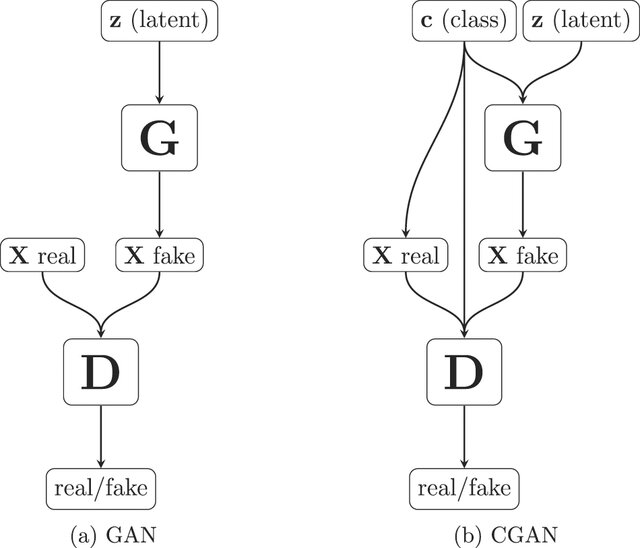
\includegraphics{schemaGAN_cGAN.jpg}
%     \caption{The general structure of GAN and cGAN networks are similar: a generator network $G$ is trained to take some noise $z$ as input to try to create a "realistic" output $X_{fake}$ and a discriminator network $D$ is trained parallelly to distinguish generated data from real data. cGAN networks introduce an information of class $c$ in the input, which is used by the generator and discriminator in their inference process. In the end, only the generator is used to create new data. }
%     \label{fig:coral-island_GAN-scheme}
% \end{figure}

% Over the past decade, deep learning has revolutionized many areas of computer graphics and procedural content creation by learning complex, data-driven priors directly from examples. Unlike purely procedural or sketch-based methods, which rely on hand-tuned noise functions or geometric constraints, neural networks can capture subtle patterns and high-frequency details without explicit programming of each effect. In terrain synthesis, this enables models to infer realistic elevation structures, textures, and region transitions from training data, even when that data is sparse or synthetic. In the context of coral-reef islands where high-resolution digital elevation models are rare, deep learning offers a way to abstract away low-level procedural rules and directly learn the mapping from semantic layouts (label maps) to plausible height fields. In the following sections, we first review general generative adversarial networks (GANs) and then focus on their conditional variant (cGAN), which forms the backbone of our sketch-to-terrain translation pipeline.

% \subsubsection{Generative Aversarial Networks}
% \label{sec:coral-island_sota-GAN}

% Generative Adversarial Networks (GANs), introduced by (\cite{Goodfellow2014}), are a class of generative models in which two neural networks are trained in opposition: a generator $G$ learns to produce synthetic data samples that resemble those from a target distribution, while a discriminator $D$ learns to distinguish real samples from those generated. Through this adversarial process, the generator improves its ability to mimic the underlying data distribution, enabling the creation of realistic outputs from random input.

% GANs have been widely adopted for image synthesis, texture generation, and data augmentation, among other tasks. In terrain modeling, they offer the potential to generate plausible landforms by learning directly from real-world data, without requiring hand-crafted procedural rules. The following works demonstrate how different GAN variants have been applied to terrain synthesis, each with its own assumptions, design trade-offs, and limitations.



% Early applications of GANs to terrain focused on unconditional generation, where elevation maps are synthesized from pure latent noise, without any spatial or semantic guidance. (\cite{WulffJensen2018}) trained a deep convolutional GAN (DCGAN) to produce realistic digital elevation models of mountainous landscapes, showing that terrain-like structures could emerge from purely data-driven learning. The model captured local elevation statistics and allowed for latent space interpolation, enabling smooth variations across generated terrains. However, the lack of spatial conditioning made it difficult to control or constrain specific features such as ridges, valleys, and coastlines, resulting in landscapes that reflected training set distributions but offered no means for intentional design.

% (\cite{Spick2019}) extended this approach by introducing a Spatial GAN that generates height and texture maps jointly. By conditioning the generation process on spatial coordinates, their model enforced local consistency and reduced structural artifacts. This integration simplified the content pipeline by fusing geometry and appearance into a single pass. Yet despite improved quality, the generation process remained fundamentally uncontrolled: there was no way for users to specify terrain layout, features, or semantics. As with earlier GANs, the model learned to mimic terrain distributions but could not support authoring or guided synthesis.

% To address the lack of control inherent in purely noise-driven GANs, later works introduced multi-stage architectures in which a second, conditional GAN refines or interprets the output of a first-stage generator. (\cite{Beckham2017}) proposed a two-step pipeline where a DCGAN generates bare terrain heightmaps from noise, and a conditional pix2pix network adds texture based on semantic cues. This separation of geometry and appearance allows for basic stylization and terrain remixing, but still suffers from the lack of control in the initial heightmap generation. In a conceptually similar structure, (\cite{Panagiotou2020}) reversed the mapping: an unconditional GAN first synthesizes aerial RGB imagery from noise, which is then passed to a cGAN trained to predict plausible DEMs. While this image-to-DEM translation enables realistic terrain reconstruction, it depends on large collections of paired data and lacks any semantic or structural control from the user. In both cases, despite the introduction of a conditional refinement stage, the generation process remains fundamentally anchored in an unconstrained latent input, offering limited authoring capability and no principled way to shape landform structures.

% These approaches show a shift toward using conditional models to guide terrain generation with more structure. But because they still start from random noise, they offer little real control over the layout or meaning of the terrain. A natural next step is to guide the generation process directly from user-defined semantic inputs, such as sketches or label maps, to produce terrain that reflects both the training data and the user's intent.


% \subsubsection{Conditional GANs for terrain generation}
% \label{sec:coral-island_sota-cGAN}

% While traditional GANs generate data from noise, Conditional GANs (cGANs) extend this concept by incorporating side information, often called class map or label map, to guide generation toward user-specified outcomes (\cite{Mirza2014}). This makes them particularly attractive for structured content synthesis tasks, including terrain generation, where user input often defines large-scale layout while realism must emerge from learned detail. The pix2pix framework by (\cite{Isola2017}) is the canonical cGAN formulation for image-to-image translation. It uses a U-Net generator conditioned on an input image (a sketch or a label map, for example), and a PatchGAN discriminator that evaluates realism at the patch level, encouraging fine detail and local consistency.

% \begin{figure}
% \centering
% 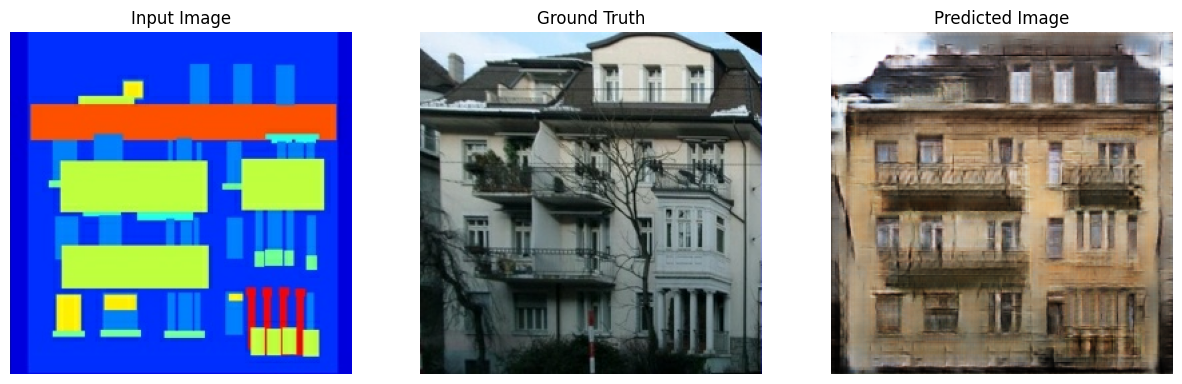
\includegraphics[width = 0.8 \linewidth]{example_pix2pix_facade.png}
% 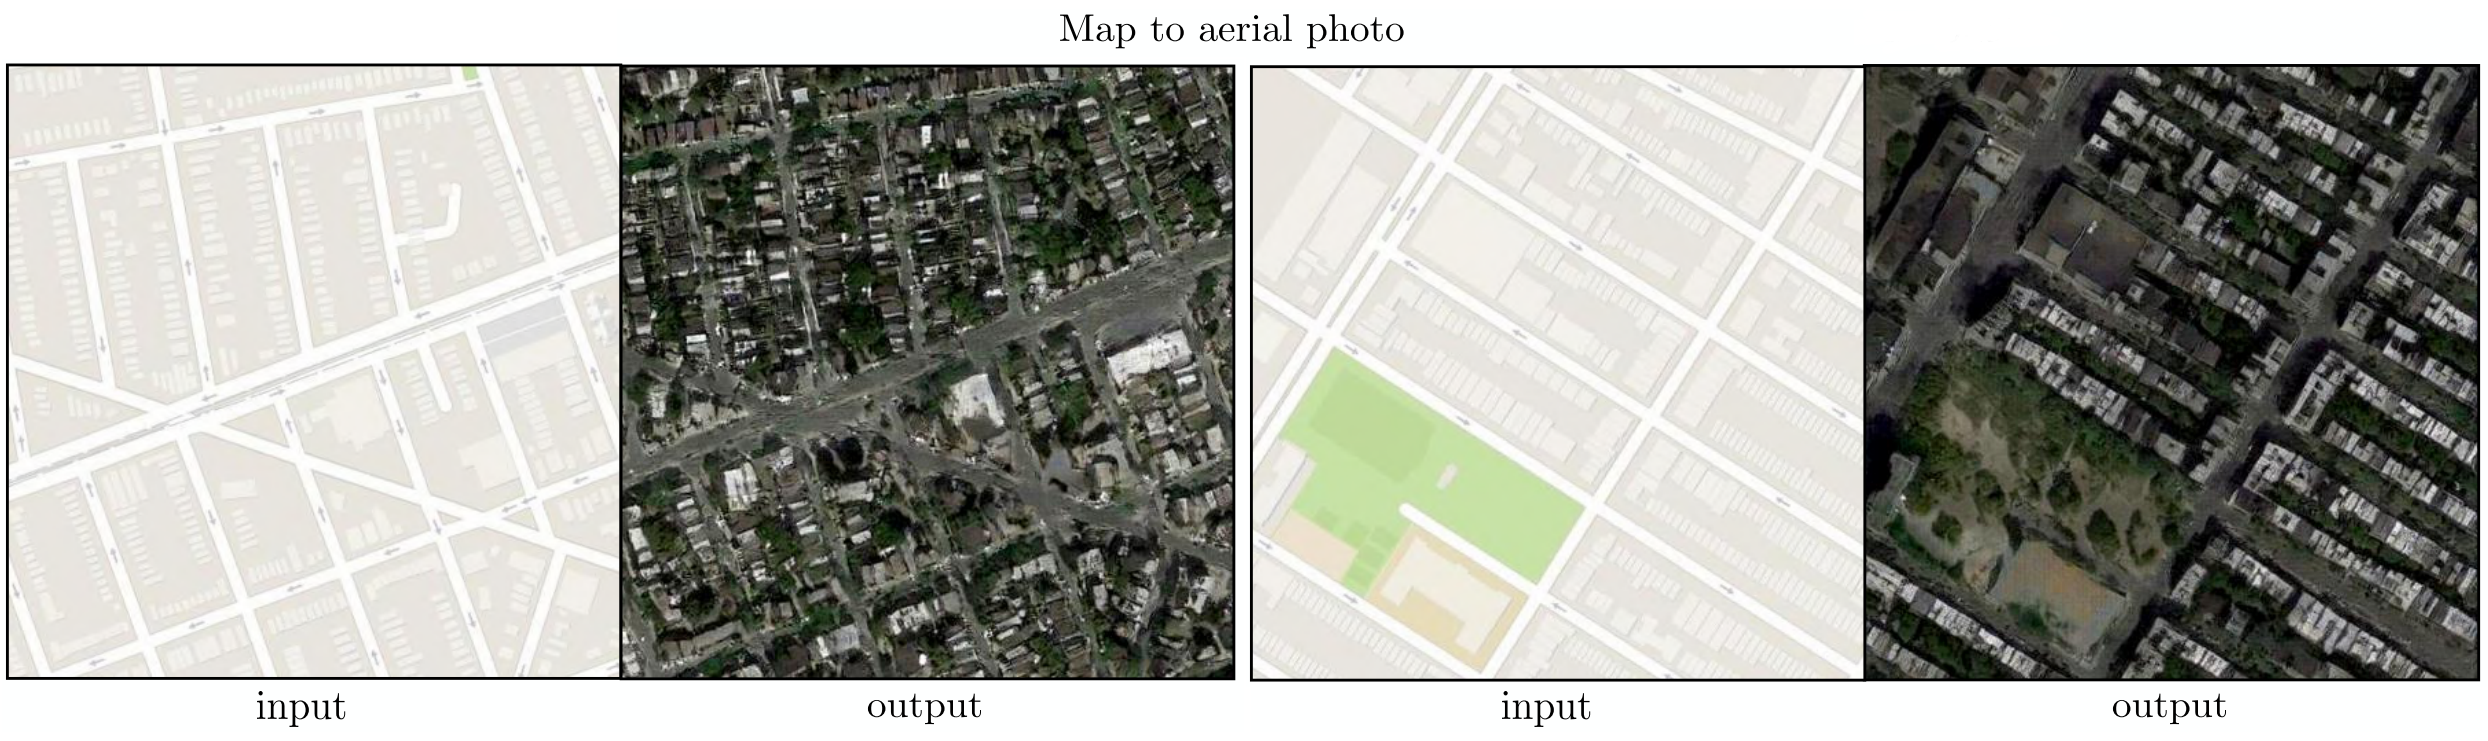
\includegraphics[width = 0.8 \linewidth]{example_pix2pix_maps.png}
% \caption{Example of pix2pix image-to-image translation: (top) a trained model converts semantic label maps into realistic façade images, or (bottom) the construction of highly plausible aerial images from navigation map sketches. This paradigm generalizes to many tasks, including terrain generation.}
% \label{fig:coral-island_pix2pix-example}
% \end{figure}

% In the domain of terrain generation, the use of cGANs remains surprisingly rare. The most directly relevant precedent is the work of (\cite{Guerin2017}), who train a pix2pix-style cGAN to map sketched terrain features such as valleys, ridgelines, or peaks, into full-resolution digital elevation models (DEMs). Their results demonstrate that cGANs can plausibly reconstruct complex topographic forms from sparse semantic cues, offering a promising balance between user control and learned realism. Similarly, (\cite{Sisodia2022}) applies a cGAN to generate stylized terrain heightmaps from sketch maps in the context of 2D game environments, further validating the sketch-to-terrain pipeline.

% Another related line of work explores learning-based terrain synthesis using partial or sparse spatial inputs. (\cite{Voulgaris2021}) propose a GAN-based system that maps sparse "altitude dot" maps to plausible terrain imagery, acting as a minimal-interaction generative authoring tool. While not strictly a cGAN, their system reflects a similar spirit: conditioning generation on lightweight user constraints. Likewise, (\cite{Panagiotou2020}) and (\cite{Beckham2017}) trained a cGAN to invert RGB satellite imagery into elevation data, framing terrain modeling as an appearance-to-geometry and geometry-to-appearance translation task. However, such image-to-DEM (and DEM-to-image) systems are heavily dependent on large paired datasets, which limits their applicability in settings like coral reef islands, where training data are scarce.

% Despite this emerging body of work, there is still no standard pipeline for generating detailed terrains from semantic layout maps using cGANs, particularly in biologically driven environments like coral reef islands. This gap is outstanding given the success of cGANs in analogous image synthesis domains, and the explosive progress in the field of deep generative models. The potential of this approach remains underexploited, especially when it comes to coupling user control with long-term geological plausibility.

% \midConclusion

% In our method, we address this gap by training a pix2pix cGAN to transform label maps (semantic region maps produced by procedural sketch-based modeling) into realistic coral reef island height fields. Each input map encodes key zones of an island (e.g., lagoon, reef crest, beach, island core) using categorical labels, serving as a semantic constraints for terrain synthesis. The cGAN generator learns to condition elevation details on both the global layout and the implicit patterns encoded in the training data. By generating our own synthetic dataset with procedurally modeled coral islands (see \cref{fig:coral-island_difficulties-dataset}), we overcome the shortage of labeled elevation data and enforce geological coherence via data generation design.

% \begin{figure}
% 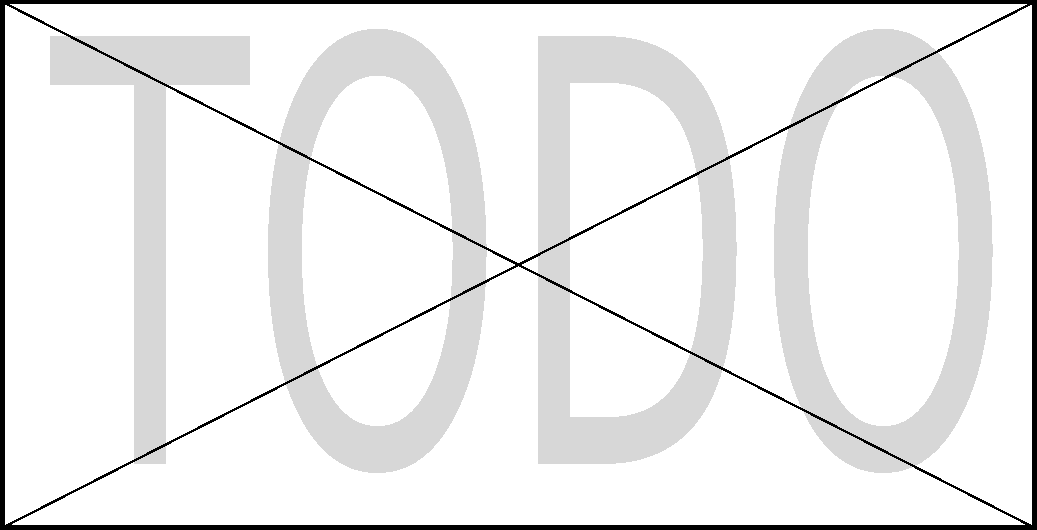
\includegraphics[width=0.9 \linewidth]{placeholder.pdf}
% \caption{Examples of procedural region maps used for training: left to right, canonical island, off-center island, elongated shapes, and multi-island scenes. These maps serve as semantic inputs to the cGAN.}
% \label{fig:coral-island_difficulties-dataset}
% \end{figure}

% This setup offers several key advantages: it respects user-defined structure while allowing the generator to introduce realistic variation, it removes procedural biases such as radial symmetry and fixed island typologies, and it enables the generation of irregular, non-circular landforms while implicitly modeling geological processes like subsidence and coral accretion through training-time priors. 

% In this context, conditional GANs emerge as a powerful yet underutilized tool for terrain modeling. By training on procedurally generated coral island data, we show that sketch-conditioned learning can effectively bridge the gap between high-level user intent and geologically plausible terrain synthesis.
